% A3 academic poster - DEM-based SAR simulation vs Sentinel-1
% Compile from poster/a3:  pdflatex poster_a3.tex
% (uses ../../report/generated/ produced by report/make_tables.py)
\documentclass[10pt]{article}
\usepackage[a3paper,portrait,margin=6mm]{geometry}
\usepackage[T1]{fontenc}
\usepackage[scaled=0.96]{helvet}
\renewcommand{\familydefault}{\sfdefault}
\usepackage{amssymb}
\usepackage{sansmath}\sansmath
\usepackage{graphicx,xcolor,booktabs,array,enumitem,pifont,calc,ragged2e}
\usepackage[most]{tcolorbox}
\usepackage{tikz}
\usetikzlibrary{positioning,arrows.meta,fit,backgrounds,calc}
\graphicspath{{../../figures/notebook/}{../../figures/pipeline/}{../../report/generated/}}
\newcommand{\dateAsc}{\textcolor{red}{[pending]}}
\newcommand{\dateDesc}{\textcolor{red}{[pending]}}
\newcommand{\geoDRmax}{\textcolor{red}{[pending]}}
\newcommand{\geoDlineMax}{\textcolor{red}{[pending]}}
\newcommand{\geoDpixMax}{\textcolor{red}{[pending]}}
\newcommand{\geoDtMax}{\textcolor{red}{[pending]}}
\newcommand{\geoidN}{\textcolor{red}{[pending]}}
\newcommand{\holesBase}{\textcolor{red}{[pending]}}
\newcommand{\holesNoOver}{\textcolor{red}{[pending]}}
\newcommand{\incAsc}{\textcolor{red}{[pending]}}
\newcommand{\incDesc}{\textcolor{red}{[pending]}}
\newcommand{\kFitDb}{\textcolor{red}{[pending]}}
\newcommand{\nFit}{\textcolor{red}{[pending]}}
\newcommand{\nGrid}{\textcolor{red}{[pending]}}
\newcommand{\nRefitDesc}{\textcolor{red}{[pending]}}
\newcommand{\platAsc}{\textcolor{red}{[pending]}}
\newcommand{\platDesc}{\textcolor{red}{[pending]}}
\newcommand{\rAsc}{\textcolor{red}{[pending]}}
\newcommand{\rDemNinety}{\textcolor{red}{[pending]}}
\newcommand{\rDesc}{\textcolor{red}{[pending]}}
\newcommand{\rDescMu}{\textcolor{red}{[pending]}}
\newcommand{\rNoOver}{\textcolor{red}{[pending]}}
\newcommand{\repoURL}{https://github.com/Vedansh7-7/dem-sar-simulation}
\newcommand{\sceneAsc}{\textcolor{red}{[pending]}}
\newcommand{\sceneDesc}{\textcolor{red}{[pending]}}
\newcommand{\shiftAscL}{\textcolor{red}{[pending]}}
\newcommand{\shiftAscP}{\textcolor{red}{[pending]}}
\newcommand{\shiftNoGeoidP}{\textcolor{red}{[pending]}}
\newcommand{\ssimAsc}{\textcolor{red}{[pending]}}
\newcommand{\ssimDesc}{\textcolor{red}{[pending]}}

\pagestyle{empty}
\setlength{\parindent}{0pt}

% ------------------------------------------------------------------ colours
\definecolor{frame}{HTML}{1F6B3A}
\definecolor{bartop}{HTML}{E9E9E9}
\definecolor{barbot}{HTML}{BEBEBE}
\definecolor{bartext}{HTML}{3A3A3A}
\definecolor{inC}{HTML}{DCE9F5}   \definecolor{inD}{HTML}{2F5F8A}
\definecolor{prC}{HTML}{E3F1E6}   \definecolor{prD}{HTML}{2E7D4A}
\definecolor{reC}{HTML}{F3EAD7}   \definecolor{reD}{HTML}{8A6A2F}
\definecolor{ouC}{HTML}{FBE3D6}   \definecolor{ouD}{HTML}{B5532A}
\definecolor{okC}{HTML}{2E7D32}   \definecolor{noC}{HTML}{C62828}

% ------------------------------------------------------------------ helpers
\newcommand{\sect}[1]{%
  \par\vspace{1.6mm}%
  \begin{tcolorbox}[enhanced,boxrule=0.5pt,colframe=barbot!75!black,arc=1.6mm,
    interior style={top color=bartop,bottom color=barbot},left=2.5mm,top=0.5mm,bottom=0.5mm,
    fontupper=\fontsize{15.5}{17.5}\selectfont\color{bartext}]#1\end{tcolorbox}\par\vspace{0.3mm}}
\newcommand{\figcap}[1]{\par\vspace{0.4mm}{\RaggedRight\fontsize{8}{9.4}\selectfont\bfseries\itshape #1\par}\vspace{0.9mm}}
\newcommand{\ok}{\textcolor{okC}{\ding{51}}}
\newcommand{\no}{\textcolor{noC}{\ding{55}}}
\setlist[itemize]{label=\scalebox{0.7}{$\blacksquare$},leftmargin=4mm,itemsep=0.8pt,topsep=0.8pt,parsep=0pt}
\newcommand{\body}{\fontsize{9.5}{11.4}\selectfont}

\begin{document}
\begin{tcolorbox}[enhanced,colback=white,colframe=frame,boxrule=2mm,arc=0mm,
  left=0mm,right=0mm,top=0mm,bottom=0mm,height=\textheight-0.5mm,valign=top]
% ================================================================== HEADER
\begin{minipage}[c]{0.715\linewidth}
\vspace{3.5mm}\hspace*{6mm}%
\begin{minipage}{\linewidth-8mm}\RaggedRight
{\fontsize{29}{33}\selectfont\bfseries DEM-based SAR Simulation and its\\Comparison with Real\\Sentinel-1 Imagery\par}
\vspace{3mm}
{\fontsize{15.5}{18}\selectfont\bfseries [Author name]\textsuperscript{*}\par}
\vspace{0.6mm}
{\fontsize{12}{14.5}\selectfont [Department, University, Country]\par}
\vspace{1.4mm}
{\fontsize{12}{14.5}\selectfont\bfseries * email: [author@university.edu]\par}
\end{minipage}
\vspace{3mm}
\end{minipage}\hfill
\begin{minipage}[c]{0.27\linewidth}\centering
\begin{minipage}[c]{0.36\linewidth}
\includegraphics[width=\linewidth]{qr_repo.png}\end{minipage}\hspace{2.5mm}%
\begin{minipage}[c]{0.56\linewidth}\raggedright\fontsize{9}{11}\selectfont
{\bfseries\color{frame} Code, notebook\\ \& data access}\\[1mm]
github.com/Vedansh7-7/\\dem-sar-simulation\\[1mm]
{\fontsize{7.5}{9}\selectfont Copernicus GLO-30 $\cdot$ Sentinel-1 $\cdot$ ESA WorldCover}\end{minipage}
\end{minipage}\hspace*{4mm}

\vspace{0.5mm}{\color{frame}\rule{\linewidth}{2mm}}
% ================================================================== BODY
\body
\hspace*{3.5mm}%
\begin{minipage}[t]{0.478\linewidth}
% ------------------------------------------------------------------ 1
\sect{1. Introduction}
\begin{minipage}[t]{0.585\linewidth}
\begin{itemize}
\item A SAR measures \textbf{slant range}: terrain height moves every point \textbf{towards the sensor} by $h\cot\theta$.
\item Slopes facing the radar are \textbf{foreshortened} or fall into \textbf{layover}; steep slopes facing away lie in \textbf{shadow} (Fig.~1).
\item Simulating the image from a DEM explains, masks and corrects these effects.
\item \textbf{Aim:} build such a simulator from first principles and test it against real Sentinel-1 data --- \emph{how much of an Alpine radar image does terrain alone explain?}
\end{itemize}
\end{minipage}\hfill
\begin{minipage}[t]{0.395\linewidth}\vspace{0pt}
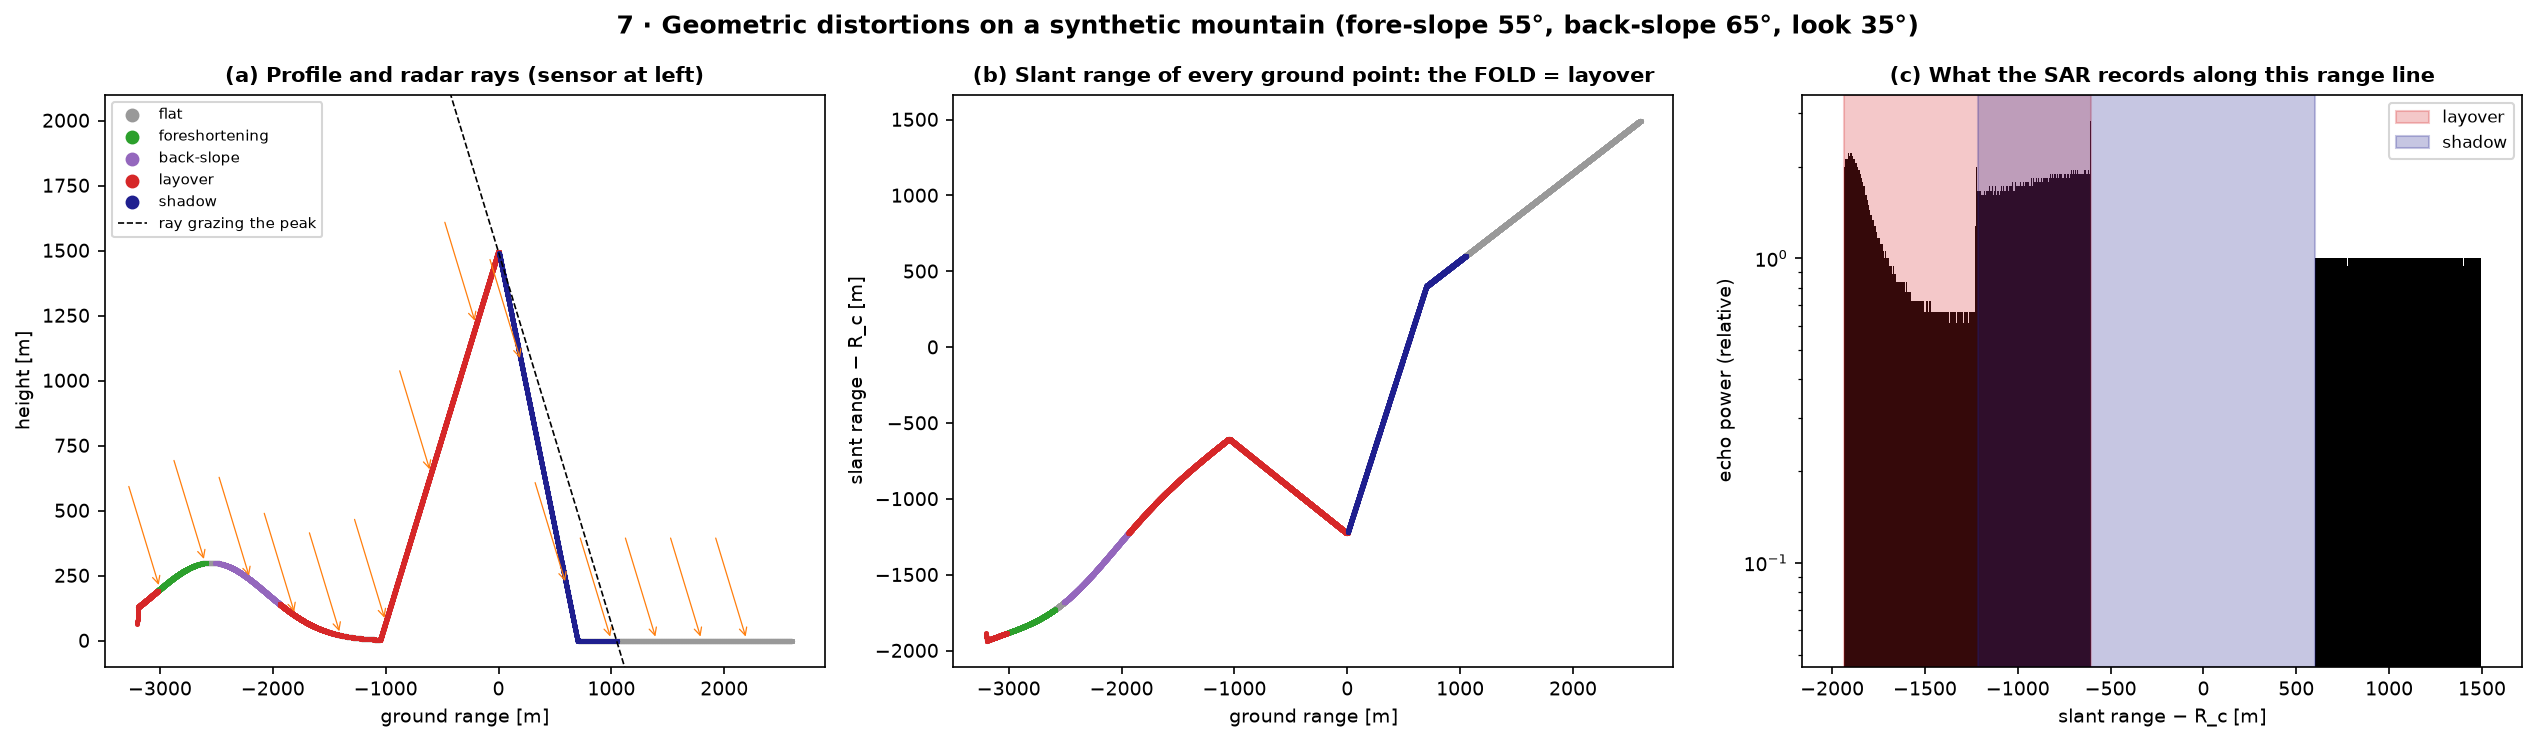
\includegraphics[width=\linewidth,trim=0 0 822 28,clip]{07_geometric_distortions_profile.png}
\figcap{Figure 1: Foreshortening (green), layover (red), shadow (blue) on a synthetic mountain; look angle 35$^\circ$.}
\end{minipage}
% ------------------------------------------------------------------ 2
\sect{2. Study Area \& Data}
\begin{minipage}[t]{0.47\linewidth}\vspace{0pt}
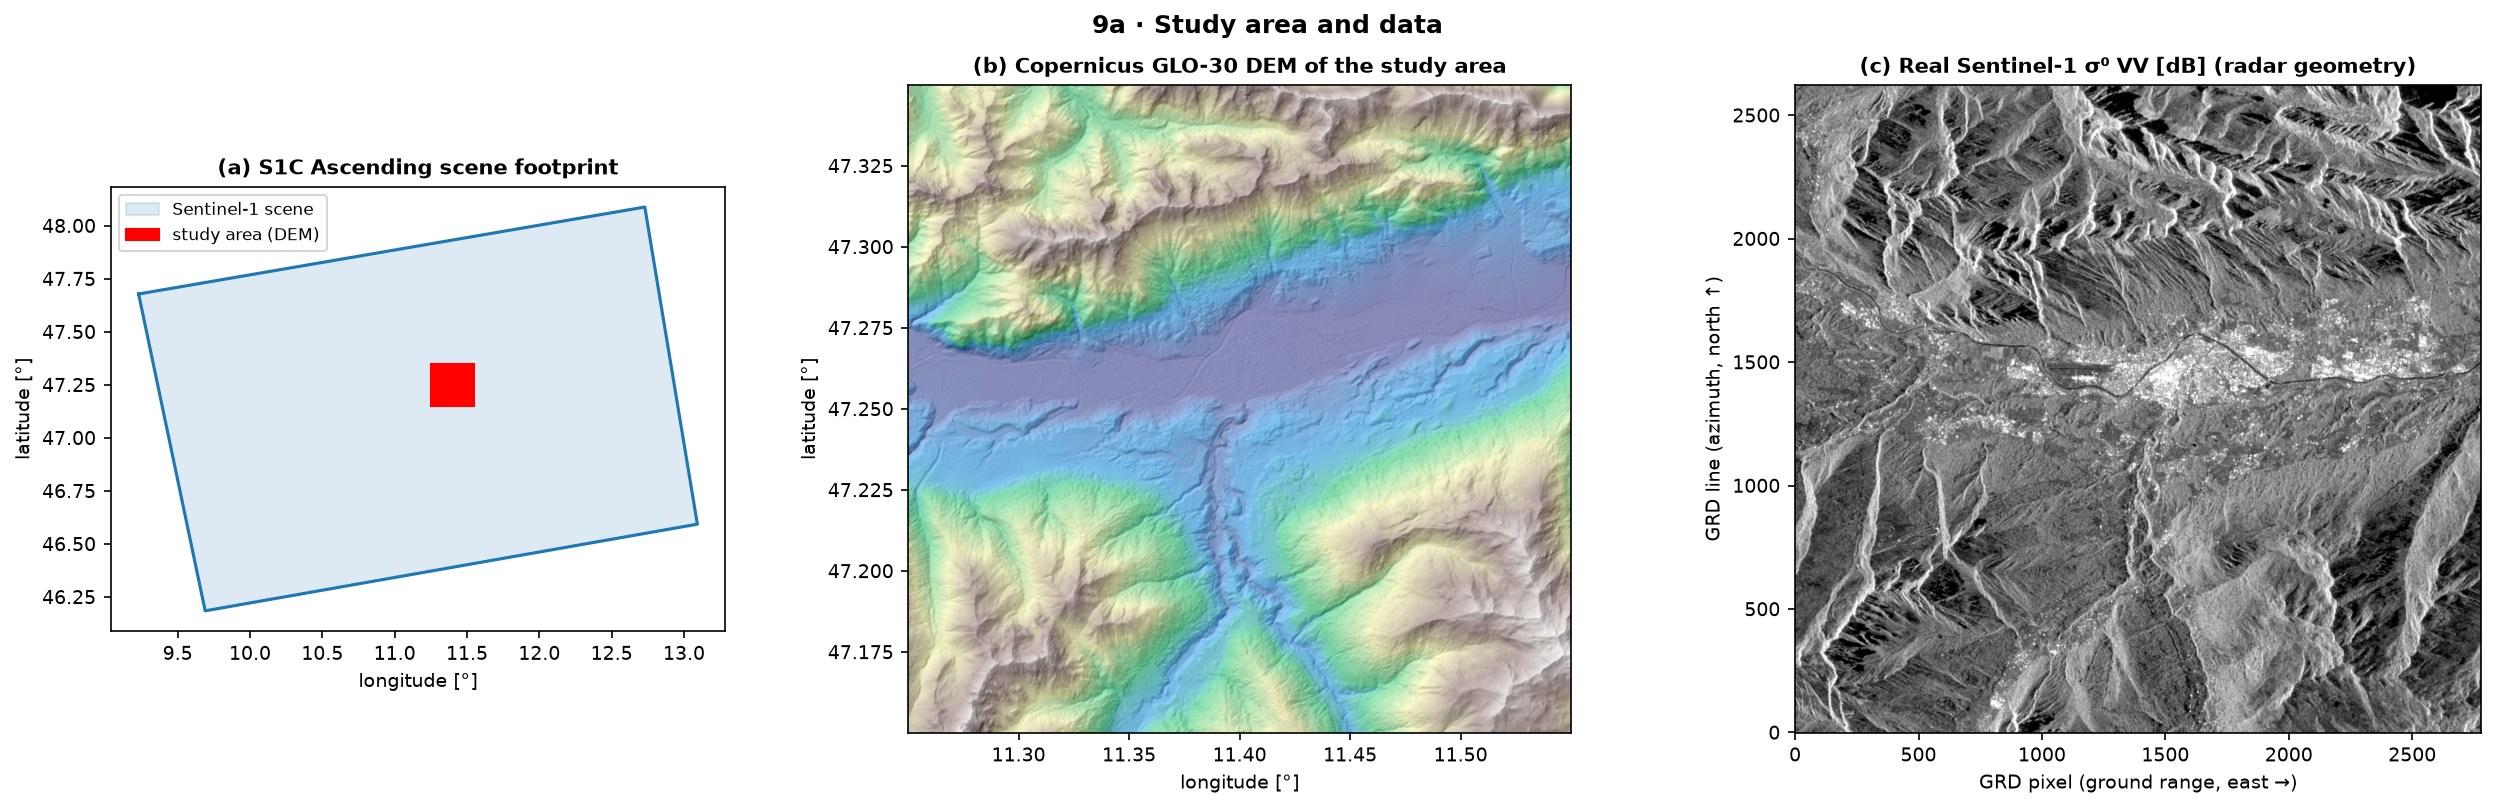
\includegraphics[width=\linewidth,trim=375 0 0 26,clip]{09a_study_area_data.png}
\figcap{Figure 2: Copernicus DEM (left) and calibrated Sentinel-1 $\sigma^0$ in radar geometry (right).}
\end{minipage}\hfill
\begin{minipage}[t]{0.51\linewidth}
\begin{itemize}
\item \textbf{Innsbruck, Austria}: Inn valley ($\approx$580\,m) between Nordkette and Patscherkofel; 23$\times$22\,km, 552--2789\,m.
\item \textbf{DEM}: Copernicus GLO-30; EGM2008 $\to$ WGS84 ($N=\geoidN$\,m).
\item \textbf{SAR}: Sentinel-1C IW GRDH VV, ascending (\dateAsc) \& descending (\dateDesc), with orbit, timing \& calibration annotation.
\item \textbf{Land cover}: ESA WorldCover 2021. All data open.
\end{itemize}
\end{minipage}
% ------------------------------------------------------------------ 3
\sect{3. Methodology}
\textbf{(a) How the simulator works.} Each DEM facet is placed in the real GRD geometry using the satellite's own orbit, given a brightness from its local incidence angle, and compared pixel by pixel with the calibrated image (Fig.~3).\par\vspace{1mm}
\centering
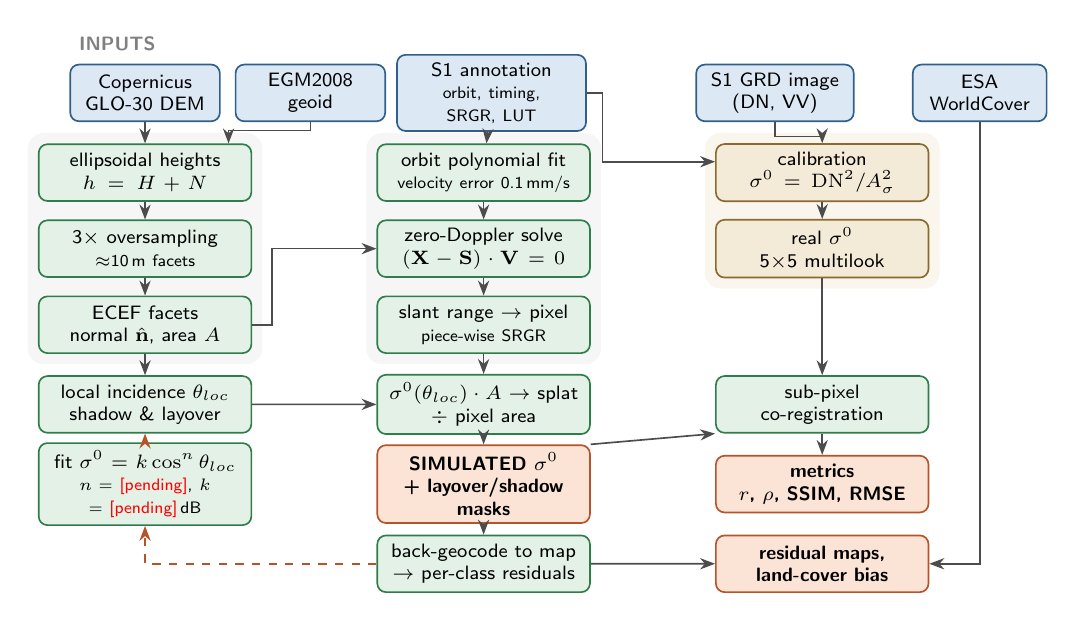
\begin{tikzpicture}[yscale=0.92,
  font=\fontsize{7}{8.1}\selectfont, >={Stealth[length=1.9mm]},
  base/.style={draw, rounded corners=1.1mm, align=center, minimum height=7.2mm, inner sep=1mm, line width=0.6pt},
  inp/.style={base, fill=inC, draw=inD, text width=19mm},
  pro/.style={base, fill=prC, draw=prD, text width=25mm},
  rea/.style={base, fill=reC, draw=reD, text width=25mm},
  prod/.style={base, fill=ouC, draw=ouD, text width=25mm, font=\fontsize{7}{8.1}\selectfont\bfseries},
  ar/.style={->, line width=0.6pt, draw=black!70},
  fb/.style={->, line width=0.75pt, draw=ouD, dashed},
  sm/.style={font=\fontsize{6.2}{7}\selectfont}]
% columns: A = DEM lane, B = orbit lane, C = real-image lane
\def\xA{0mm} \def\xB{43mm} \def\xC{86mm}
% ---- inputs
\node[inp, text width=17mm] (dem) at (\xA,0) {Copernicus\\GLO-30 DEM};
\node[inp, text width=17mm] (geo) at (21mm,0) {EGM2008\\geoid};
\node[inp, text width=22mm] (ann) at (\xB+1mm,0) {S1 annotation\\{\fontsize{6.2}{7}\selectfont orbit, timing, SRGR, LUT}};
\node[inp, text width=18mm] (grd) at (\xC-6mm,0) {S1 GRD image\\(DN, VV)};
\node[inp, text width=15mm] (wc) at (\xC+20mm,0) {ESA\\WorldCover};
% ---- row 1..3
\node[pro] (hgt)  at (\xA,-11mm) {ellipsoidal heights\\$h=H+N$};
\node[pro] (orb)  at (\xB,-11mm) {orbit polynomial fit\\{\fontsize{6.2}{7}\selectfont velocity error 0.1\,mm/s}};
\node[rea] (cal)  at (\xC,-11mm) {calibration\\$\sigma^0=\mathrm{DN}^2/A_\sigma^2$};
\node[pro] (ovs)  at (\xA,-21.5mm) {3$\times$ oversampling\\{\fontsize{6.2}{7}\selectfont $\approx$10\,m facets}};
\node[pro] (zd)   at (\xB,-21.5mm) {zero-Doppler solve\\$(\mathbf X-\mathbf S)\cdot\mathbf V=0$};
\node[rea] (rml)  at (\xC,-21.5mm) {real $\sigma^0$\\5$\times$5 multilook};
\node[pro] (ecef) at (\xA,-32mm) {ECEF facets\\normal $\hat{\mathbf n}$, area $A$};
\node[pro] (srgr) at (\xB,-32mm) {slant range $\to$ pixel\\{\fontsize{6.2}{7}\selectfont piece-wise SRGR}};
% ---- row 4..6
\node[pro] (inc)  at (\xA,-43mm) {local incidence $\theta_{loc}$\\shadow \& layover};
\node[pro] (spl)  at (\xB,-43mm) {$\sigma^0(\theta_{loc})\cdot A$ $\to$ splat\\$\div$ pixel area};
\node[pro] (reg)  at (\xC,-43mm) {sub-pixel\\co-registration};
\node[pro] (fit)  at (\xA,-54mm) {fit $\sigma^0=k\cos^n\theta_{loc}$\\{\fontsize{6.2}{7}\selectfont $n$ = \nFit, $k$ = \kFitDb\,dB}};
\node[prod] (sim) at (\xB,-54mm) {SIMULATED $\sigma^0$\\+ layover/shadow masks};
\node[prod] (met) at (\xC,-54mm) {metrics\\$r$, $\rho$, SSIM, RMSE};
\node[pro]  (map) at (\xB,-65mm) {back-geocode to map\\$\to$ per-class residuals};
\node[prod] (res) at (\xC,-65mm) {residual maps,\\land-cover bias};
% ---- arrows
\draw[ar] (dem) -- (hgt);
\draw[ar] (geo.south) |- ($(hgt.north east)+(-3mm,1.8mm)$) -- ++(0,-1.8mm);
\draw[ar] (hgt) -- (ovs);
\draw[ar] (ovs) -- (ecef);
\draw[ar] (ann) -- (orb);
\draw[ar] (orb) -- (zd);
\draw[ar] (zd) -- (srgr);
\draw[ar] (ecef.east) -- ++(2.5mm,0) |- (zd.west);
\draw[ar] (ecef) -- (inc);
\draw[ar] (srgr) -- (spl);
\draw[ar] (inc) -- (spl);
\draw[ar] (spl) -- (sim);
\draw[ar] (grd.south) -- ++(0,-2mm) -| (cal.north);
\draw[ar] (ann.east) -- ++(2mm,0) |- ($(cal.west)+(0,1.5mm)$);
\draw[ar] (cal) -- (rml);
\draw[ar] (rml) -- (reg);
\draw[ar] (sim.north east) -- (reg.south west);
\draw[ar] (reg) -- (met);
\draw[ar] (sim) -- (map);
\draw[ar] (map) -- (res);
\draw[ar] (wc.south) |- (res.east);
\draw[fb] (map.west) -| (fit.south);
\draw[fb] (fit.north) -- (inc.south);
\node[font=\fontsize{6.8}{8}\selectfont\bfseries\color{black!50}, anchor=south west] at ($(dem.north west)+(0,0.5mm)$) {INPUTS};
\begin{scope}[on background layer]
  \node[fill=black!3.5, rounded corners=2mm, fit=(hgt)(ovs)(ecef), inner sep=1.3mm] {};
  \node[fill=black!3.5, rounded corners=2mm, fit=(orb)(zd)(srgr), inner sep=1.3mm] {};
  \node[fill=reC!45, rounded corners=2mm, fit=(cal)(rml), inner sep=1.3mm] {};
\end{scope}
\end{tikzpicture}
\figcap{Figure 3: Data flow. Blue: inputs; green: simulation; beige: real-image path; orange: products. Dashed: the backscatter law is fitted to the real image and fed back into the simulation.}
\justifying
\textbf{(b) How the final design was reached.} The simulator was grown in nine iterations. Each had to pass a quantitative test before the next was built; every failed test (\no) forced a design decision that is now part of the pipeline (Fig.~4).\par\vspace{1mm}
\centering
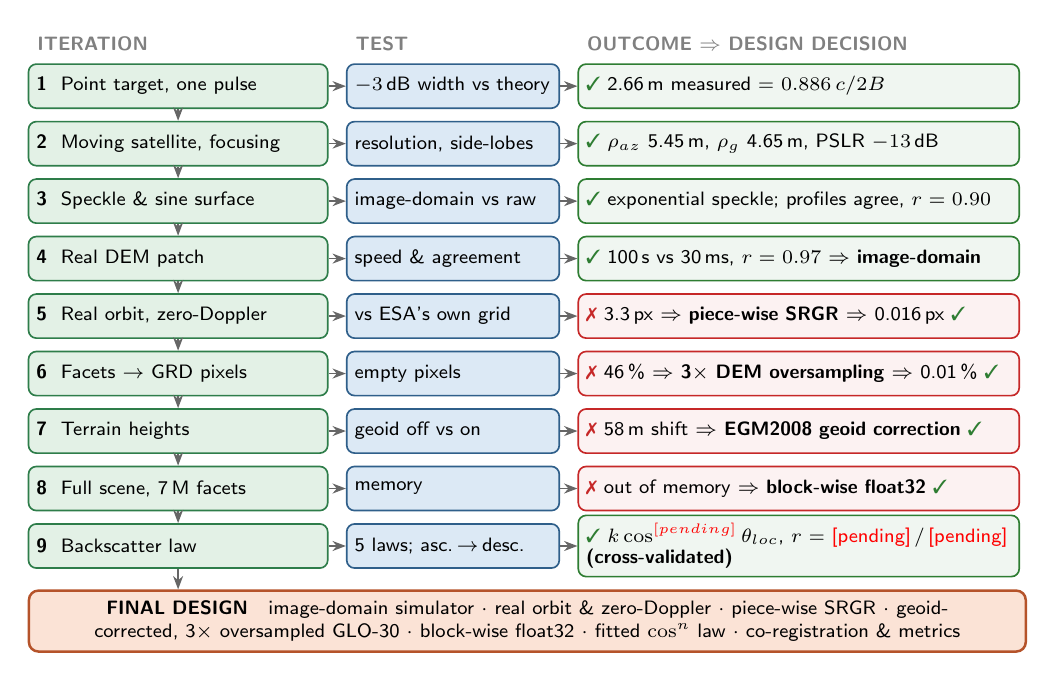
\begin{tikzpicture}[font=\fontsize{6.9}{7.9}\selectfont, >={Stealth[length=1.7mm]},
  st/.style={draw=prD, fill=prC, rounded corners=1mm, line width=0.6pt, text width=36mm, minimum height=5.6mm, align=left, inner sep=1mm},
  te/.style={draw=inD, fill=inC, rounded corners=1mm, line width=0.6pt, text width=25mm, minimum height=5.6mm, align=left, inner sep=1mm},
  okb/.style={draw=okC, fill=okC!7, rounded corners=1mm, line width=0.6pt, text width=54mm, minimum height=5.6mm, align=left, inner sep=1mm},
  nob/.style={draw=noC, fill=noC!6, rounded corners=1mm, line width=0.6pt, text width=54mm, minimum height=5.6mm, align=left, inner sep=1mm},
  ar/.style={->, line width=0.55pt, draw=black!60}]
\def\dy{7.3mm}
\foreach \i/\stage/\test/\res/\kind in {
  1/{\textbf{1}\ \ Point target, one pulse}/{$-3$\,dB width vs theory}/{\ok\ 2.66\,m measured = $0.886\,c/2B$}/okb,
  2/{\textbf{2}\ \ Moving satellite, focusing}/{resolution, side-lobes}/{\ok\ $\rho_{az}$ 5.45\,m, $\rho_g$ 4.65\,m, PSLR $-13$\,dB}/okb,
  3/{\textbf{3}\ \ Speckle \& sine surface}/{image-domain vs raw}/{\ok\ exponential speckle; profiles agree, $r=0.90$}/okb,
  4/{\textbf{4}\ \ Real DEM patch}/{speed \& agreement}/{\ok\ 100\,s vs 30\,ms, $r=0.97$ $\Rightarrow$ \textbf{image-domain}}/okb,
  5/{\textbf{5}\ \ Real orbit, zero-Doppler}/{vs ESA's own grid}/{\no\ 3.3\,px $\Rightarrow$ \textbf{piece-wise SRGR} $\Rightarrow$ 0.016\,px \ok}/nob,
  6/{\textbf{6}\ \ Facets $\to$ GRD pixels}/{empty pixels}/{\no\ 46\,\% $\Rightarrow$ \textbf{3$\times$ DEM oversampling} $\Rightarrow$ 0.01\,\% \ok}/nob,
  7/{\textbf{7}\ \ Terrain heights}/{geoid off vs on}/{\no\ 58\,m shift $\Rightarrow$ \textbf{EGM2008 geoid correction} \ok}/nob,
  8/{\textbf{8}\ \ Full scene, 7\,M facets}/{memory}/{\no\ out of memory $\Rightarrow$ \textbf{block-wise float32} \ok}/nob,
  9/{\textbf{9}\ \ Backscatter law}/{5 laws; asc.\,$\to$\,desc.}/{\ok\ $k\cos^{\nFit}\theta_{loc}$, $r$ = \rAsc\,/\,\rDesc\ \textbf{(cross-validated)}}/okb}{
  \node[st] (s\i) at (0,-\i*\dy) {\stage};
  \node[te, right=2.2mm of s\i] (t\i) {\test};
  \node[\kind, right=2.2mm of t\i] (r\i) {\res};
  \draw[ar] (s\i) -- (t\i);
  \draw[ar] (t\i) -- (r\i);
}
\foreach \i [count=\j from 2] in {1,...,8} { \draw[ar] (s\i) -- (s\j); }
\node[draw=ouD, fill=ouC, line width=0.9pt, rounded corners=1.2mm, align=center, inner sep=1.3mm,
      anchor=north west, font=\fontsize{7.2}{8.4}\selectfont, text width=124mm] (fin) at ($(s9.south west)+(0,-2.6mm)$)
  {\textbf{FINAL DESIGN}\quad image-domain simulator $\cdot$ real orbit \& zero-Doppler $\cdot$ piece-wise SRGR $\cdot$ geoid-corrected, 3$\times$ oversampled GLO-30 $\cdot$ block-wise float32 $\cdot$ fitted $\cos^{n}$ law $\cdot$ co-registration \& metrics};
\draw[ar] (s9) -- (s9|-fin.north);
\node[font=\fontsize{6.8}{8}\selectfont\bfseries\color{black!50}, anchor=south west] at ($(s1.north west)+(0,0.4mm)$) {ITERATION};
\node[font=\fontsize{6.8}{8}\selectfont\bfseries\color{black!50}, anchor=south west] at ($(t1.north west)+(0,0.4mm)$) {TEST};
\node[font=\fontsize{6.8}{8}\selectfont\bfseries\color{black!50}, anchor=south west] at ($(r1.north west)+(0,0.4mm)$) {OUTCOME $\Rightarrow$ DESIGN DECISION};
\end{tikzpicture}
\figcap{Figure 4: Design evolution. Green: test passed; red: test failed, and the fix that became part of the final design.}
\end{minipage}\hfill
{\color{frame}\vrule width 1.3mm}\hfill
\begin{minipage}[t]{0.478\linewidth}
% ------------------------------------------------------------------ 4
\sect{4. Results}
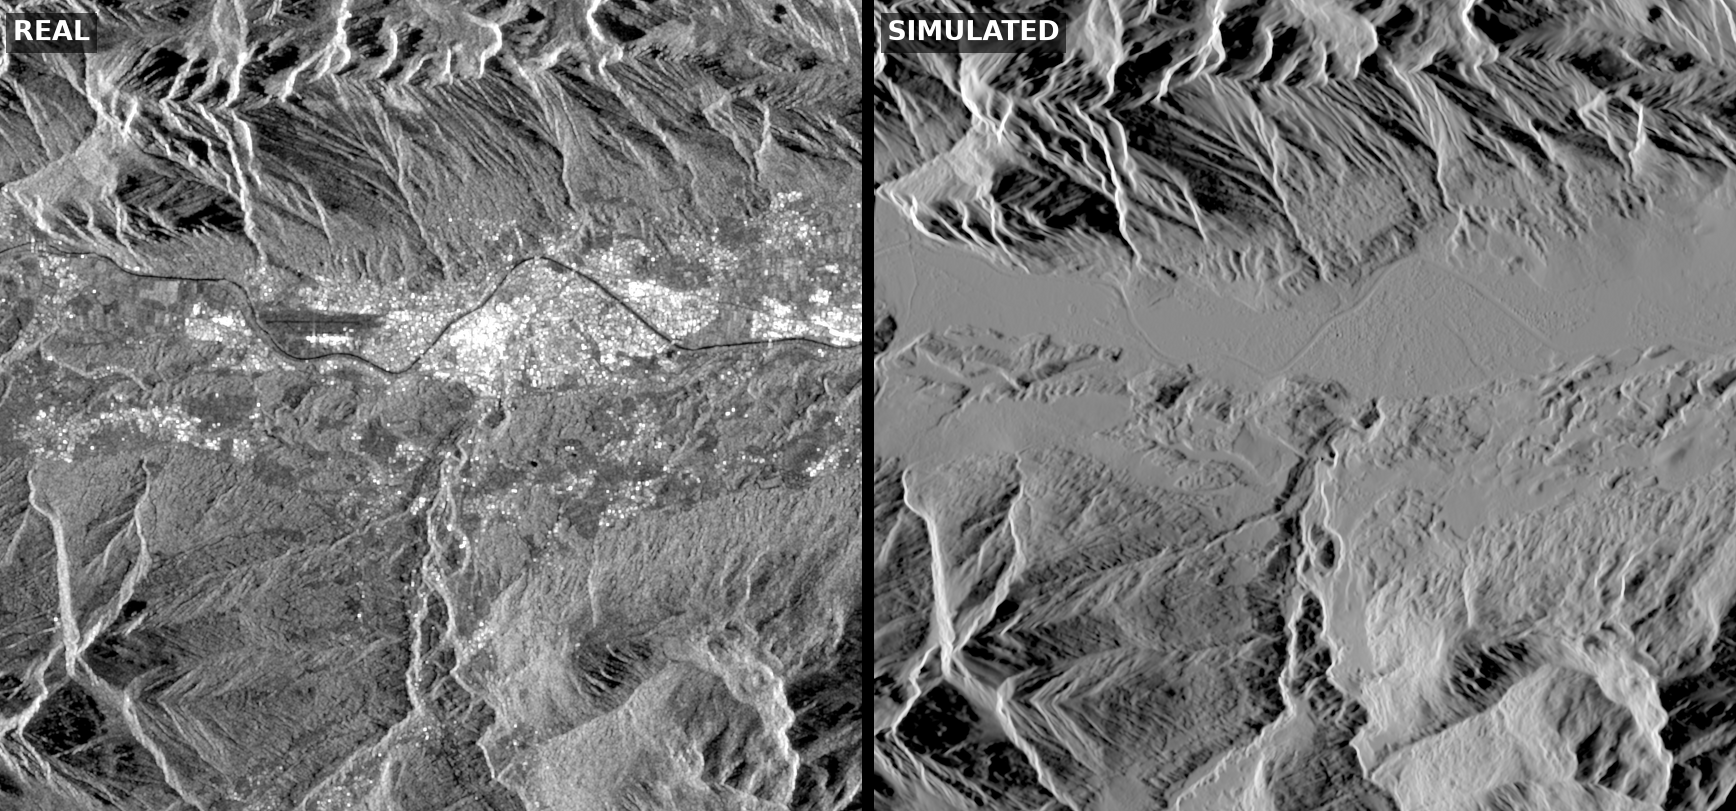
\includegraphics[width=\linewidth]{p0_hero.png}
\figcap{Figure 5: Real (left) and simulated (right) Sentinel-1 $\sigma^0$ VV, ascending pass, radar geometry, north up.}
\begin{itemize}
\item \textbf{Geometry:} range-Doppler geocoding reproduces ESA's geolocation grid to \textbf{\geoDpixMax\,px} in range and \geoDtMax\,ms in azimuth time; predicted layover and shadow fall on the real bright and dark features in \emph{both} orbit directions (Fig.~6).
\item \textbf{Agreement:} Pearson $r$ = \textbf{\rAsc} (ascending) and \textbf{\rDesc} (descending, with the law fitted on ascending only); SSIM \ssimAsc\,/\,\ssimDesc; \nPix\,M pixels.
\end{itemize}\vspace{0.6mm}
\begin{minipage}[t]{0.305\linewidth}\vspace{0pt}
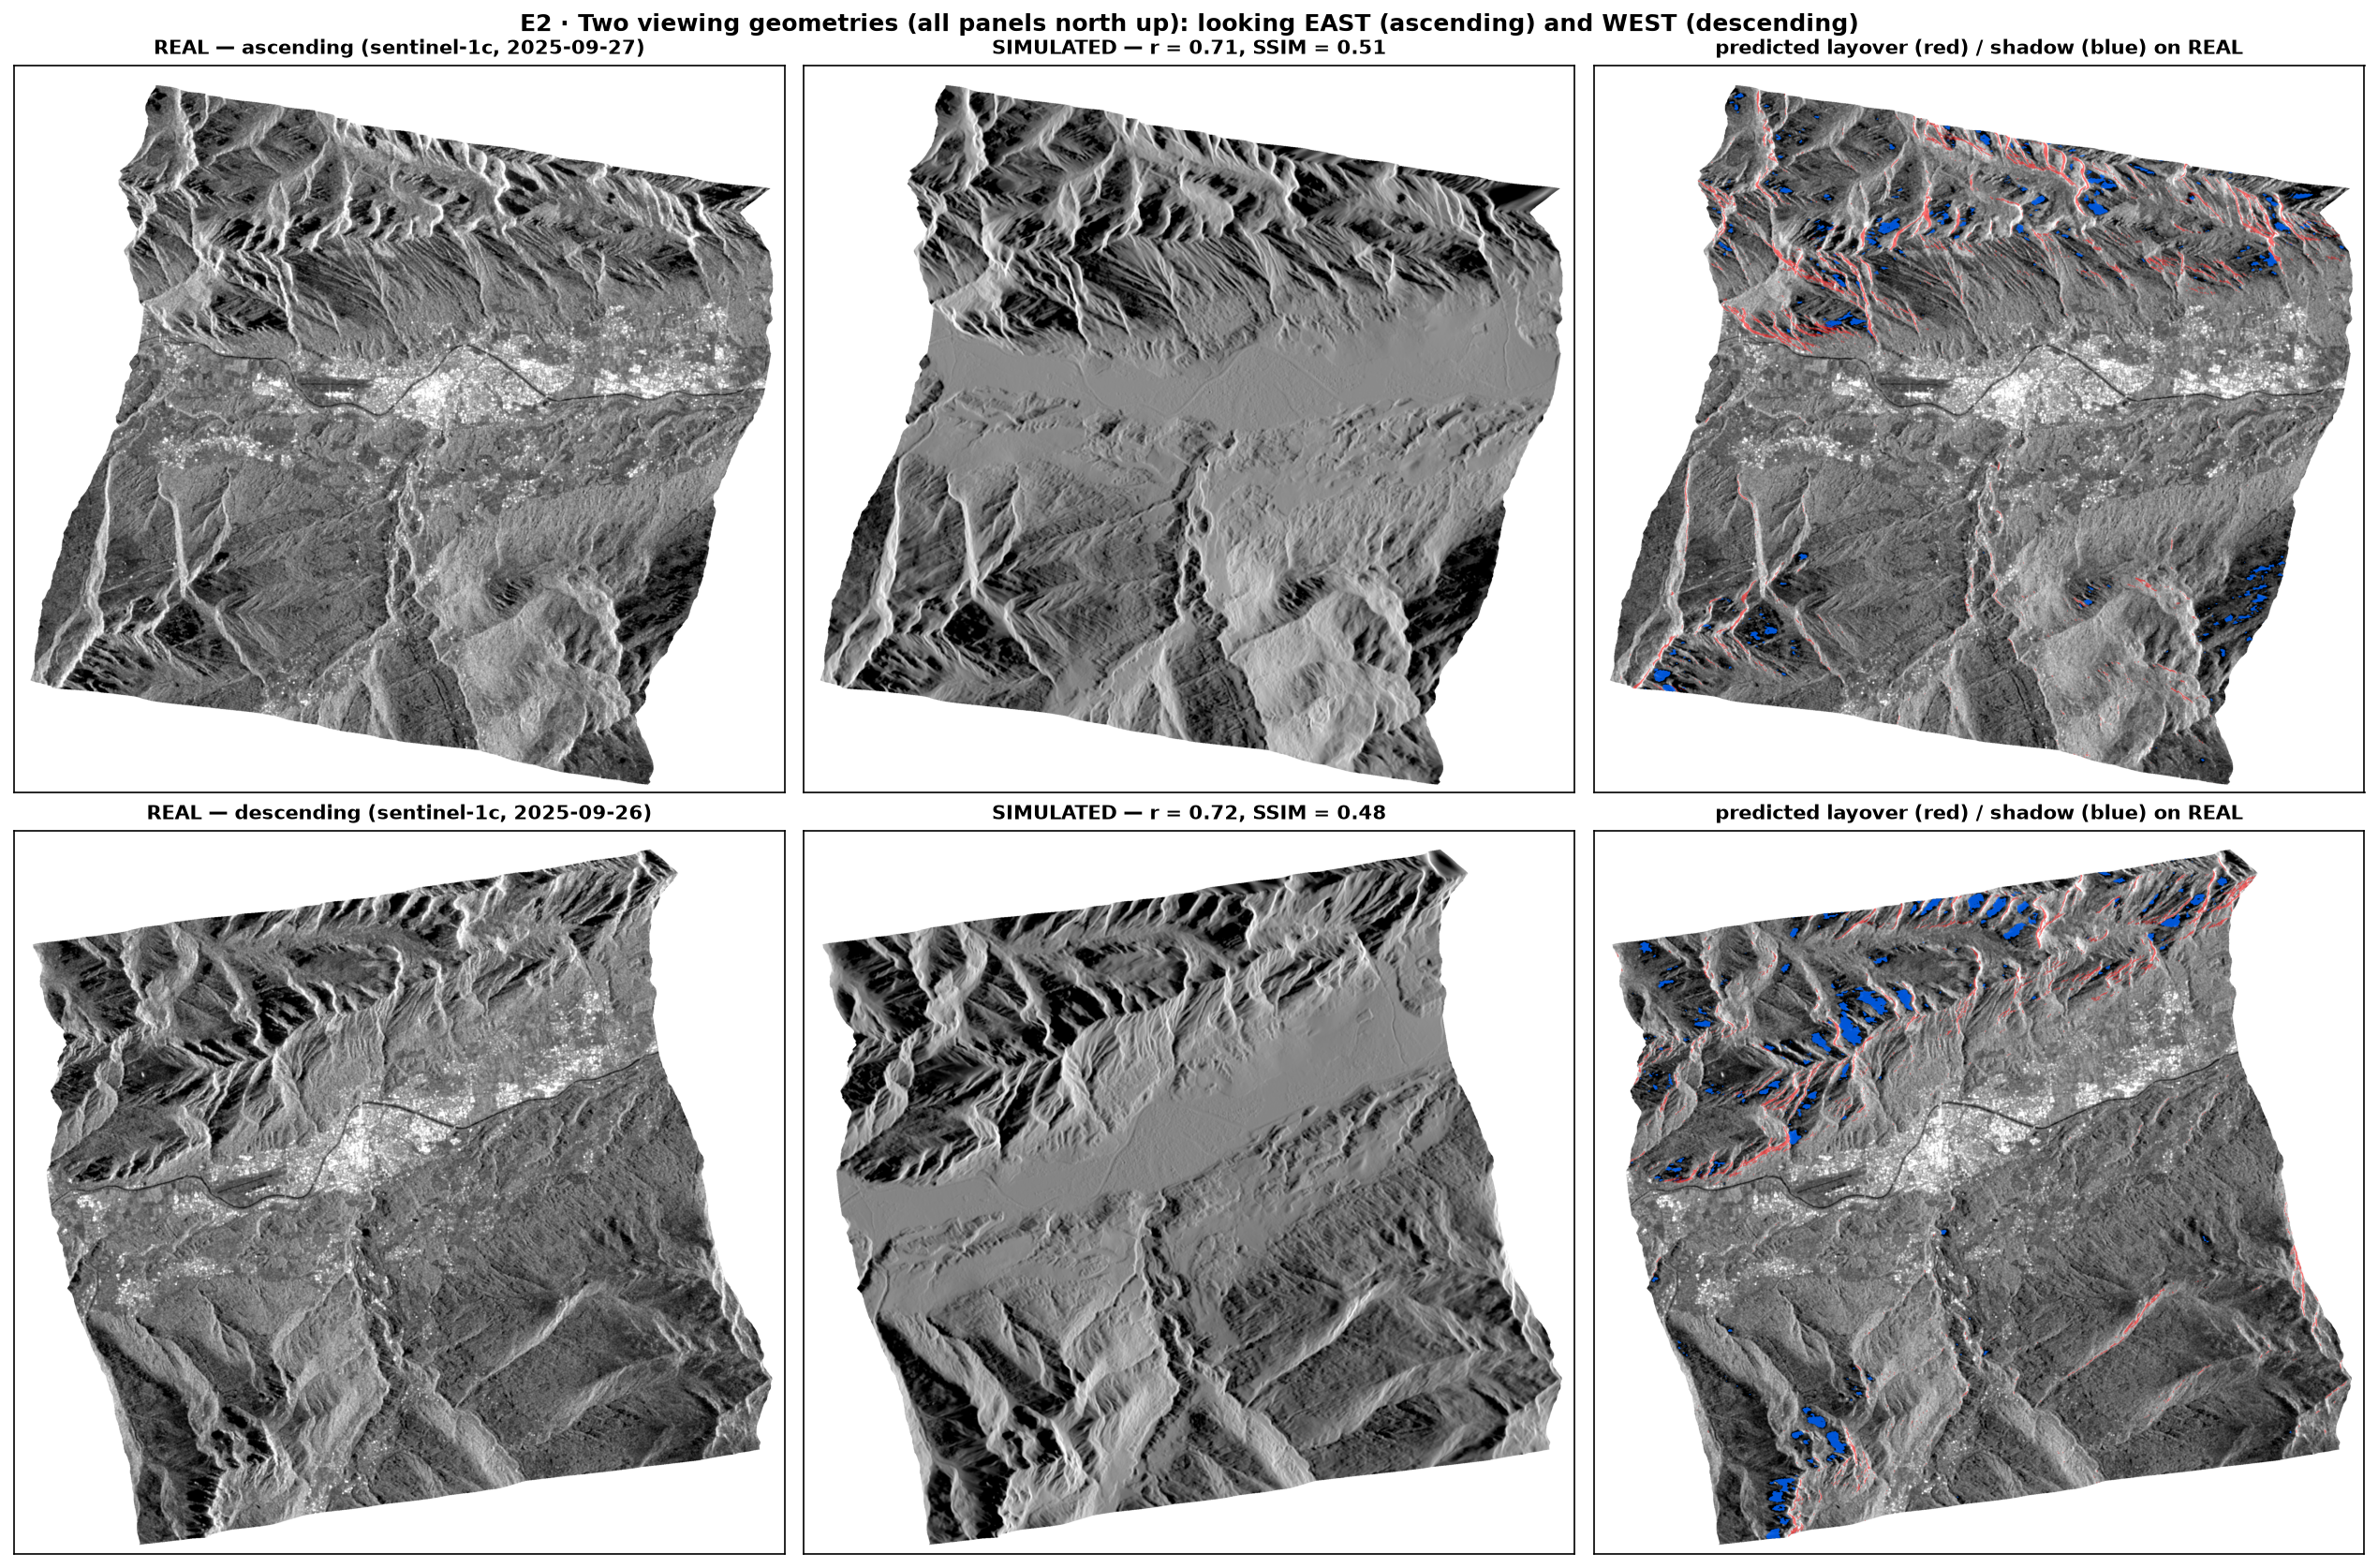
\includegraphics[width=\linewidth,trim=820 0 0 24,clip]{p3_ascending_descending.png}
\figcap{Figure 6: Predicted layover (red) and shadow (blue) on the real image; ascending (top, looking east), descending (bottom, looking west).}
\end{minipage}\hfill
\begin{minipage}[t]{0.675\linewidth}\vspace{0pt}
{\setlength{\tabcolsep}{2pt}\resizebox{\linewidth}{!}{\begin{tabular}{lrrrrr}\toprule
 Backscatter model & Pearson $r$ & Spearman $\rho$ & SSIM & RMSE [dB] & level offset [dB]\\\midrule
Constant & 0.534 & 0.739 & 0.377 & 3.83 & -0.6 \\
$\cos\theta_{loc}$ & 0.663 & 0.767 & 0.467 & 3.72 & -8.3 \\
$\cos^2\theta_{loc}$ (Lambert) & 0.703 & 0.762 & 0.509 & 4.44 & -6.1 \\
Muhleman & 0.734 & 0.757 & 0.494 & 4.58 & 7.6 \\
Fitted $k\cos^{1.98}\theta_{loc}$ & 0.710 & 0.761 & 0.508 & 4.29 & -1.4 \\
\bottomrule\end{tabular}
}\par}
\figcap{Table 1: Five backscatter laws (ascending, dB, 5$\times$5 looks).}
{\setlength{\tabcolsep}{2pt}\resizebox{\linewidth}{!}{\begin{tabular}{lrrrr}\toprule
 & \multicolumn{2}{c}{ascending} & \multicolumn{2}{c}{descending}\\
Predicted class & pixels & median $\sigma^0$ [dB] & pixels & median $\sigma^0$ [dB]\\\midrule
shadow & 47k & -21.0 & 66k & -22.0 \\
layover & 82k & -3.5 & 61k & -3.9 \\
foreshortened (area > 2x) & 228k & -4.5 & 220k & -5.1 \\
other terrain & 4525k & -10.8 & 4576k & -11.5 \\
\bottomrule\end{tabular}
}\par}
\figcap{Table 2: Real $\sigma^0$ inside the predicted classes.}
\begin{itemize}
\item Geometry alone (constant law) already gives $r\approx0.53$.
\item Muhleman reaches the highest $r$, Lambert-like laws the highest SSIM; the law fitted to the data is $\cos^{\nFit}\theta\approx$ Lambert and transfers to the other orbit.
\item Predicted shadow sits at the noise floor ($\approx-21$\,dB); layover is brightest.
\item Image offsets of $\le$35\,m reflect the products' absolute geolocation, not the simulator.
\end{itemize}
\end{minipage}
\vspace{0.4mm}
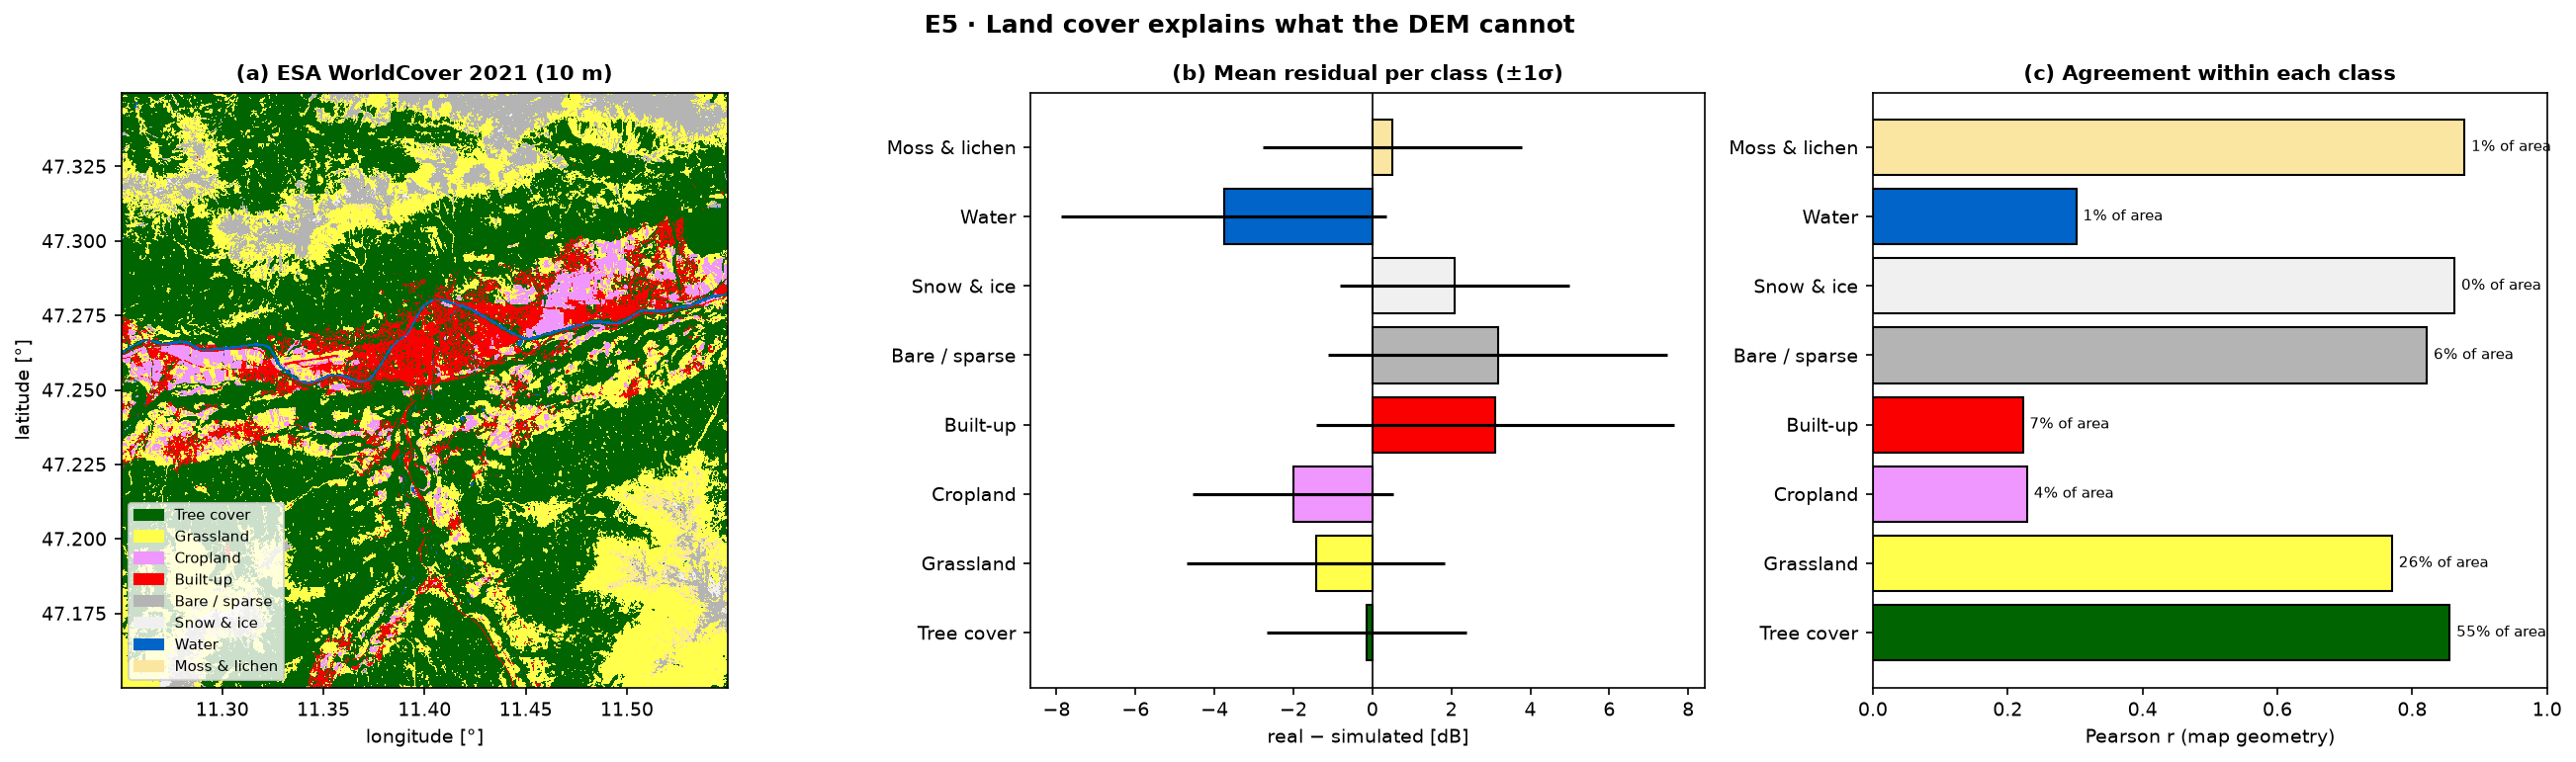
\includegraphics[width=\linewidth,trim=0 0 0 30,clip]{p6_landcover.png}
\figcap{Figure 7: Residual (real $-$ simulated) per land-cover class: forest (55\,\% of the area) fits without bias; built-up and bare rock are $\approx$3\,dB brighter, water $\approx$4\,dB darker.}
% ------------------------------------------------------------------ 5
\sect{5. Conclusions}
\begin{itemize}
\item A SAR simulator grown from a single point target to a full scene predicts real Sentinel-1 images of Alpine terrain with $r$ = \rAsc\ / \rDesc, using only a DEM and the product's own orbit.
\item Geometry is solved to hundredths of a pixel; the remaining disagreement is \textbf{land cover} --- double bounce in the city, specular water, rough rock --- which a DEM cannot know.
\item Next: land-cover-dependent backscatter, double bounce, radiometric terrain flattening, simulation-based co-registration.
\end{itemize}
\begin{minipage}[t]{0.595\linewidth}
\sect{References}
{\RaggedRight\fontsize{7.6}{9}\selectfont
Cumming \& Wong (2005). \textit{Digital Processing of SAR Data}. Artech House.\\
Moreira et al. (2013). A tutorial on SAR. \textit{IEEE GRSM} 1(1), 6--43.\\
Small (2011). Flattening gamma. \textit{IEEE TGRS} 49(8), 3081--3093.\\
Muhleman (1964). Radar scattering from Venus and the Moon. \textit{Astron.\ J.} 69, 34--41.\par}
\end{minipage}\hfill
\begin{minipage}[t]{0.385\linewidth}
\sect{Acknowledgements}
{\RaggedRight\fontsize{7.6}{9}\selectfont Copernicus DEM \textcopyright\ ESA/Airbus; Sentinel-1 \& WorldCover \textcopyright\ ESA, Copernicus Programme; data via Microsoft Planetary Computer.\par}
\end{minipage}
\end{minipage}\hspace*{3.5mm}
\end{tcolorbox}
\end{document}
